\documentclass[tikz,border=1pt]{standalone}
% Shared style of the Background schematics (bg_*.tex).  Colors follow figures/bar_patterns.py: each hue keeps one
% meaning across the paper (light blue with a blue outline = active / required position, green = WISEConv, red = the baseline
% frames, dotted gray = wasted computation, as in fig:gap).  Drawn at \columnwidth (241 pt), included unscaled.  Cell fills and
% the dark-navy rules come from the authors' original schematics (input C1E5F5, now a light lavender E2DCEE so that it stays apart from the blue active cells; weights a light yellow F6E2A6);
% the SM fill is a lighter step of their D9D9D9 so that it stays apart from the wasted gray.
\usepackage[T1]{fontenc}
\usepackage[tt=false,type1=true]{libertine}
\usepackage[libertine]{newtxmath}
\usepackage{tikz}
\usetikzlibrary{arrows.meta,calc,patterns.meta,positioning,fit,backgrounds,decorations.pathreplacing}

\definecolor{ink}{HTML}{222222}
\definecolor{muted}{HTML}{6B6B68}
\definecolor{rule}{HTML}{2A4552}
\definecolor{wiseconv}{HTML}{2A7F4A}
\definecolor{tileskip}{HTML}{5F7C97}
\definecolor{gather}{HTML}{7F98AF}
\definecolor{wasted}{HTML}{DDDDDD}
\definecolor{wastedink}{HTML}{9A9A9A}
\definecolor{baseline}{HTML}{C0392B}  % the baseline frames (red)
\definecolor{infill}{HTML}{E2DCEE}
\definecolor{wfill}{HTML}{F6E2A6}
\definecolor{smfill}{HTML}{EAEAEA}
\definecolor{actfill}{HTML}{D2E1F7}
\definecolor{actred}{HTML}{2A64C0}  % active positions: light blue fill, blue outline (2026-11-16 palette: green ours, red baselines, blue active)
\colorlet{gsfill}{gather!45!white}

\tikzset{
  every picture/.style={line join=round, line cap=round, font=\fontsize{8}{9.6}\selectfont, color=ink},
  cell/.style={draw=rule, line width=0.35pt, minimum size=#1, inner sep=0pt, outer sep=0pt, anchor=north west},
  cell/.default=3.6mm,
  idx/.style={font=\fontsize{6.8}{7}\selectfont, text=ink!85},
  act/.style={fill=actfill},
  inp/.style={fill=infill},
  wgt/.style={fill=wfill},
  waste/.style={fill=wasted, postaction={pattern={Dots[distance=1.2pt, radius=0.22pt]}, pattern color=wastedink}},
  gs/.style={fill=gsfill},
  sm/.style={fill=smfill, rounded corners=2pt, draw=none},
  mem/.style={fill=white, draw=rule, line width=0.4pt, rounded corners=1.2pt},
  smlabel/.style={font=\fontsize{6.8}{7}\selectfont\scshape, text=muted, anchor=north west, inner sep=1.4pt},
  flow/.style={-{Stealth[length=3.2pt, width=2.6pt]}, line width=0.55pt, draw=ink},
  title/.style={font=\fontsize{8}{9}\selectfont, anchor=north, inner sep=1pt},
  op/.style={font=\fontsize{9.5}{10}\selectfont, text=ink},
}

% \grid{x}{y}{cols}{rows}{size}{style of cell i (macro taking the index)}{first index label or empty}
% \actbox <path>; fills an active cell and outlines it in red on a layer above the grid lines
\pgfdeclarelayer{actlayer}
\pgfsetlayers{background,main,actlayer}
\def\actbox#1;{\fill[actfill] #1;\begin{pgfonlayer}{actlayer}\draw[actred, line width=0.6pt] #1;\end{pgfonlayer}}

\newcommand{\cellat}[4]{% x, y (top-left), size, style
  \node[cell=#3, #4] at (#1, #2) {};}

% \figframe{baseline|ours}{tag}: an outer frame around the whole schematic, placed last in the tikzpicture.  Baselines
% (fig:masked-conv, fig:tile-skip, fig:gather-scatter) get a dashed purple frame, WISEConv (fig:overview) a solid orange
% one, each with its tag on the top edge.  Colors and widths follow the frames of the intro figure (fig:teaser, purple
% Dense and orange WISEConv, 2026-11-15): both 0.9 pt, read off the figure at \columnwidth (about 5 px of 1280).
\tikzset{
  baselineframe/.style={draw=baseline, line width=0.9pt, dash pattern=on 2.4pt off 1.4pt, rounded corners=3pt},
  oursframe/.style={draw=wiseconv, line width=0.9pt, rounded corners=3pt},
  baselinetag/.style={fill=white, inner xsep=1.4pt, inner ysep=0.6pt, anchor=west, text=baseline!70!black,
                      font=\fontsize{7.4}{8}\selectfont\bfseries},
  ourstag/.style={baselinetag, text=wiseconv!80!black},
}
\newcommand{\figframe}[2]{%
  \coordinate (ff-sw) at ($(current bounding box.south west)+(-0.9,-0.9)$);
  \coordinate (ff-ne) at ($(current bounding box.north east)+(0.9,2.0)$);
  \draw[#1frame] (ff-sw) rectangle (ff-ne);
  \node[#1tag] at ($(ff-sw|-ff-ne)+(3.0,0)$) {#2};}

% fig:masked-conv: a 3x3 convolution on a 4x4 grid, drawn as the Dense row of the intro figure (fig:teaser): the input
% x with its padding ring, the receptive fields N(p) of all 16 positions laid out as the grid of positions (the four
% corners N(0), N(3), N(12), N(15) drawn, the rest elided; the 3x3 window of N(0) is dashed on x), the weights f, and
% the output y with the output mask, whose active positions 0, 5, 9, 12, 14 are the running example of fig:tile-skip
% and fig:gather-scatter.
\begin{document}
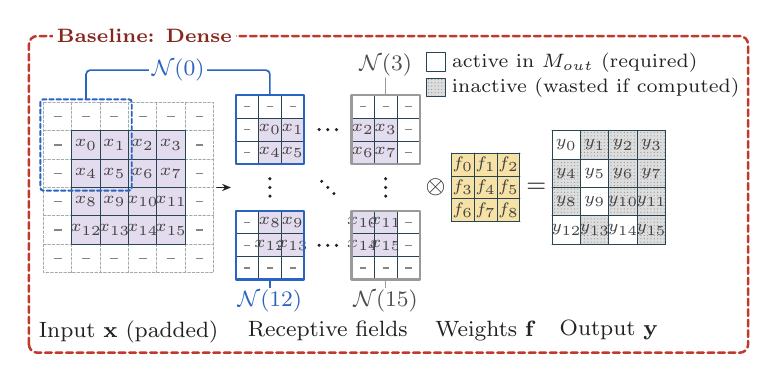
\begin{tikzpicture}[x=1mm, y=1mm, idx/.append style={font=\fontsize{6.4}{6.8}\selectfont}]
  \def\c{3.6}                                     % cell of x and y
  \def\pc{2.9}                                    % cell of a receptive field and of f
  \def\isact#1{\pgfmathparse{or(or(or(or(#1==0,#1==5),#1==9),#1==12),#1==14)}}
  \tikzset{small idx/.style={idx, font=\fontsize{5.7}{6.1}\selectfont},
           window/.style={line width=0.7pt, dash pattern=on 1.6pt off 1pt, rounded corners=1pt}}
  \def\pad{-}\def\actcol{actred}
  % cells are filled first and their grid lines drawn once afterwards, so that shared edges keep one width
  % \padmark{center x}{center y}{half length}: the padding mark, a short rule at the cell's exact center
  \newcommand{\padmark}[3]{\draw[ink!55, line width=0.5pt, line cap=butt] ({#1-#3}, #2) -- ({#1+#3}, #2);}
  % \rf{x}{y}{nine entries, row-major; - is padding}{frame color}: one receptive field
  \newcommand{\rf}[4]{%
    \foreach \e [count=\k from 0] in {#3} {
      \pgfmathtruncatemacro\r{\k/3}\pgfmathtruncatemacro\q{mod(\k,3)}
      \ifx\e\pad
        \fill[white] (#1+\q*\pc, #2-\r*\pc) rectangle ++(\pc, -\pc);
        \padmark{#1+\q*\pc+\pc/2}{#2-\r*\pc-\pc/2}{0.4}
      \else
        \fill[infill] (#1+\q*\pc, #2-\r*\pc) rectangle ++(\pc, -\pc);
        \node[small idx] at (#1+\q*\pc+\pc/2, #2-\r*\pc-\pc/2) {$x_{\e}$};
      \fi}
    \foreach \k in {1,2} \draw[rule, line width=0.35pt] (#1+\k*\pc, #2) -- ++(0, -3*\pc) (#1, #2-\k*\pc) -- ++(3*\pc, 0);
    \draw[#4, line width=0.8pt] (#1, #2) rectangle ++(3*\pc, -3*\pc);}
  % input x inside its padding ring (padded grid 6x6, x at rows/columns 1-4)
  \begin{scope}[shift={(0,-0.9)}]
  \begin{scope}[rule!45, line width=0.35pt, dash pattern=on 0.9pt off 0.7pt]
    \draw (0, 0) rectangle (6*\c, -6*\c);
    \foreach \k in {1,...,5} \draw (\k*\c, 0) -- ++(0, -\c) (\k*\c, -5*\c) -- ++(0, -\c)
                                   (0, -\k*\c) -- ++(\c, 0) (5*\c, -\k*\c) -- ++(\c, 0);
  \end{scope}
  \foreach \i in {0,...,5} \foreach \j in {0,...,5} {
    \pgfmathtruncatemacro\inside{and(and(\i>0,\i<5),and(\j>0,\j<5))}
    \ifnum\inside=0 \padmark{\i*\c+\c/2}{-\j*\c-\c/2}{0.5}\fi}
  \foreach \i in {0,...,15} {
    \pgfmathtruncatemacro\r{\i/4}\pgfmathtruncatemacro\q{mod(\i,4)}
    \fill[infill] (\c+\q*\c, -\c-\r*\c) rectangle ++(\c, -\c);
    \node[idx] at (\c+\q*\c+\c/2, -\c-\r*\c-\c/2) {$x_{\i}$};
  }
  \foreach \k in {0,...,4} \draw[rule, line width=0.35pt] (\c+\k*\c, -\c) -- ++(0, -4*\c) (\c, -\c-\k*\c) -- ++(4*\c, 0);
  % the 3x3 window of N(0), padding included, drawn just outside its nine cells
  \draw[actred, window] (-0.4, 0.4) rectangle ++(3*\c+0.8, -3*\c-0.8);
  \end{scope}
  \draw[flow] (22.0,-11.7) -- (23.8,-11.7);
  % receptive fields in the layout of the positions: N(0) ... N(3) / ... / N(12) ... N(15)
  \rf{24.4}{0}{-,-,-,-,0,1,-,4,5}{actred}
  \rf{39.1}{0}{-,-,-,2,3,-,6,7,-}{wastedink}
  \rf{24.4}{-14.7}{-,8,9,-,12,13,-,-,-}{actred}
  \rf{39.1}{-14.7}{10,11,-,14,15,-,-,-,-}{wastedink}
  % ellipses as three dots centered in the gaps (the TeX glyphs sit off center)
  \foreach \x/\y/\a in {36.1/-4.35/0, 36.1/-19.05/0, 28.75/-11.7/90, 43.45/-11.7/90, 36.1/-11.7/-45}
    \foreach \k in {-1,0,1} \fill[ink] ($(\x,\y)+(\a:\k*1.1)$) circle (0.22);
  % labels of the drawn receptive fields
  \draw[actred, line width=0.6pt, rounded corners=1.5pt] (5.4, -0.5) -- (5.4, 3.2) -- (28.75, 3.2) -- (28.75, 0.0);
  \node[fill=white, inner sep=1pt, text=actred] at (17.1, 3.2) {$\mathcal{N}(0)$};
  \draw[wastedink, line width=0.5pt] (43.45, 0.0) -- (43.45, 2.2);
  \node[anchor=south, inner sep=0.6pt, text=ink!80] at (43.45, 2.2) {$\mathcal{N}(3)$};
  % receptive fields of active outputs (0 and 12) in red, the others in gray
  \foreach \x/\n/\col in {28.75/12/actred, 43.45/15/wastedink} {
    \draw[\col, line width=0.5pt] (\x, -23.4) -- (\x, -24.4);
    \node[anchor=north, inner sep=0.6pt, text=\ifx\col\actcol actred\else ink!80\fi] at (\x, -24.4) {$\mathcal{N}(\n)$};}
  % weights f
  \foreach \i in {0,...,8} {
    \pgfmathtruncatemacro\r{\i/3}\pgfmathtruncatemacro\q{mod(\i,3)}
    \fill[wfill] (51.8+\q*\pc, -7.35-\r*\pc) rectangle ++(\pc, -\pc);
    \node[small idx] at (51.8+\q*\pc+\pc/2, -7.35-\r*\pc-\pc/2) {$f_{\i}$};
  }
  \foreach \k in {0,...,3} \draw[rule, line width=0.35pt] (51.8+\k*\pc, -7.35) -- ++(0, -3*\pc) (51.8, -7.35-\k*\pc) -- ++(3*\pc, 0);
  % output y with the mask
  \begin{scope}[shift={(64.6,-4.5)}]
    \foreach \i in {0,...,15} {
      \pgfmathtruncatemacro\r{\i/4}\pgfmathtruncatemacro\q{mod(\i,4)}
      \isact{\i}
      \ifnum\pgfmathresult=1 \actbox (\q*\c, -\r*\c) rectangle ++(\c, -\c);
      \else \path[waste] (\q*\c, -\r*\c) rectangle ++(\c, -\c); \fi
      \node[idx] at (\q*\c+\c/2, -\r*\c-\c/2) {$y_{\i}$};
    }
    \foreach \k in {0,...,4} \draw[rule, line width=0.35pt] (\k*\c, 0) -- ++(0, -4*\c) (0, -\k*\c) -- ++(4*\c, 0);
  \end{scope}
  \node[op] at (49.8, -11.7) {$\otimes$};
  \node[op] at (62.6, -11.7) {$=$};
  % labels
  \node[title] at (10.8, -28.2) {Input $\mathbf{x}$ (padded)};
  \node[title] at (36.1, -28.2) {Receptive fields};
  \node[title] at (56.15, -28.2) {Weights $\mathbf{f}$};
  \node[title] at (71.8, -28.2) {Output $\mathbf{y}$};
  % legend, top right
  \begin{scope}[shift={(48.6, 5.4)}, every node/.style={font=\fontsize{7}{8}\selectfont, anchor=north west, align=left, inner sep=0.5pt}]
    \actbox (0, 0) rectangle ++(2.4, -2.4); \draw[rule, line width=0.35pt] (0, 0) rectangle ++(2.4, -2.4);
    \node at (3.0, 0.2) {active in $M_{out}$ (required)};
    \path[waste] (0, -3.2) rectangle ++(2.4, -2.4); \draw[rule, line width=0.35pt] (0, -3.2) rectangle ++(2.4, -2.4);
    \node at (3.0, -3.0) {inactive (wasted if computed)};
  \end{scope}
  \figframe{baseline}{Baseline: Dense}
\end{tikzpicture}
\end{document}
